\documentclass{report}
\usepackage[margin=1in]{geometry}
\usepackage{setspace}
\usepackage{times}
\title{
	\textsc{ \small
		Washington State University \\
		School of Electrical Engineering and Computer Science \\
		EE 352, Electrical Engineering Laboratory
	} \\
	{\textsc{\small Lab \#1}} \\
	Equipment Familiarity and First Order Electrical Circuits
}

\author{
	Name: Kevin Evans \\
	Partner: Jacob Hnatiak
}
\date{Due Date: January 28, 2020}


% start sections at 1 with subsections to 1.1, 1.2...
\renewcommand{\thesection}{\arabic{section}}
\newcommand{\pp}{_{pp}}
\newcommand{\Vpp}{\V\pp}

\usepackage{siunitx}
\usepackage{threeparttable}
\usepackage{booktabs}
\usepackage{multirow}
\usepackage{graphicx}
\usepackage{float}
\begin{document}

\maketitle
\section*{Lab Overview}
In this lab, we regained familiarity with the function generator and oscilloscope and determined the functional limitations of each. From this, we experimented with the various settings of the function generator and digital multimeter (DMM). It was found the internal shunt impedances of the oscilloscope and DMM can greatly affect measurements. Next, we validated the behavior of a first-order series RL circuit. Each circuit was built and tested and compared to the expected simulation. We then characterized the internal impedance of the 1X and 10X oscilloscope probes as a first-order RC circuit and found the limitations of it.


\section{Function generator and oscilloscope}
\subsection{Purpose}
The purpose of this experiment was to regain familiarity with the function generator and oscilloscope and to determine the limitations of each piece of equipment. 

\subsection{Theoretical background}
The equipment used in the lab has several limitations: particularly in the frequencies and amplitudes the oscilloscope and function generator can read and produce. It is important to note these limitations for future experiments. The function generator (Rigol DG1022Z) has several limits set in the software, later listed in Table \ref{table:exp1}.

\subsection{Procedure}
The following steps were carried out as instructed by the lab assignment.
\begin{enumerate}
	\item[0.] Take inventory of the equipment used.
	\item Two 1X BNC coaxial leads were teed from the output of the function generator and connected to CH1 and CH2 of the oscilloscope. For each available waveform (sinusoidal, square pulse, and triangular pulse), the frequency was swept from the minimum (\SI{1}{\micro\Hz}) to its maximum (\SI{25}{\mega\Hz}).
	\item Next, a similar procedure was done with the peak-to-peak amplitudes varied.
	\item This readability of each was recorded.
	\item A \SI{10}{\V} peak-to-peak sine wave was generated at \SI{10}{\kilo\Hz}. The peak voltage was recorded, using both the time/div feature and the measure function on the oscilloscope. This data was recorded.
	\item A \SI{5}{\V} DC offset was added to the signal and the DC/AC coupling was explored in the oscilloscope.
\end{enumerate}

\subsection{Results and analysis}
The equipment used in this lab are noted in Table \ref{table:exp0}. In the first step of the procedure, an output waveform was teed into two channels on the oscilloscope. It was found that the signals were identical, as expected. The oscilloscope has a theoretical maximum of \SI{100}{\mega\Hz} and the function generator has a functional range of \SI{1}{\micro\Hz} to \SI{25}{\mega\Hz}. As for the amplitudes, the function generator has a minimum of \SI{1}{\milli\V} and a maximum of \SI{10}{\V} (peak). However, the smaller frequencies and voltages cannot be observed on the oscilloscope as the waveforms are too deteriorated, as noted by Table \ref{table:exp1}.

Using the time/div feature (eyeballing), the \SI{10}{\Vpp} signal was found to be \SI{10}{\Vpp}. Using the measure feature of the oscilloscope, it was found as \SI{10.2}{\Vpp}.

\subsection{Conclusion}
There are several limitations of the equipment that we must be aware of. The measurement tool within the scope has several inadequacies, and it can be better to eyeball or to use cursors when measuring \si{\Vpp} signals.

\pagebreak
\hspace{0pt}
\vfill

\begin{table}[H]
	\centering
	\caption{Inventory of the lab equipment used in this experiment.}
	\begin{threeparttable}
		\label{table:exp0}
		\begin{tabular}{cc}
			\toprule
			Item & Model \\
			\midrule
			Oscilloscope & Tektronix TDS2014B \\
			Digital Multimeter (DMM) & Fluke 45 \\
			Function Generator & Rigol DG1022Z \\
			Power Supply & DP832 \\
			\bottomrule
		\end{tabular}
	\end{threeparttable}
\end{table}

\begin{table}[H]
	\centering
	\caption{Observed minimum and maximum limits of the Rigol DG1022Z function generator and Tek TDS2014B oscilloscope.}
	\begin{threeparttable}
		\label{table:exp1}
		\begin{tabular}{cccc}
			\toprule
			& Limit & Observed Frequency (Theoretical) & Obs. Amplitude (Theoretical) \\
			\midrule
			\multirow{2}{*}{\textbf{Function generator}} & Min. & \SI{100}{\micro\Hz} (\SI{1}{\micro\Hz}) & \SI{100}{\milli\V} (\SI{1}{\milli\volt}) \\
			& Max. & \SI{25}{\MHz} & \SI{10}{\V} \\
			\midrule
			\multirow{2}{*}{\textbf{Oscilloscope}} & Min. & (DC) & (\SI{1}{\mV}) \\
			& Max. & (\SI{100}{\MHz}) & (\SI{300}{\V} RMS, \SI{13}{\Vpp} at \SI{3}{\MHz}) \\
			\bottomrule
		\end{tabular}
		\begin{tablenotes}
			\item \footnotesize Note: the theoretical values, listed within the parenthesis, are noted from the respective datasheets.
		\end{tablenotes}
	\end{threeparttable}
\end{table}

\vfill
\hspace{0pt}
\pagebreak


\section{Digital multimeter (DMM) verses the Oscilloscope}
\subsection{Purpose}
This experiment demonstrated the differences in measurement between the digital multimeter (DMM) and the oscilloscope, due to the internal impedance of both.
\subsection{Theoretical background}
Both the DMM and the oscilloscope have an internal impedance that can greatly affect the measurements. The scope has two probes available, the 1X and 10X probe, which have different impedances. The varying impedances can reduce the effect that the probe has on the circuit. Here, we model the different impedances with a parallel resistor and capacitor.
\subsection{Procedure}
\begin{enumerate}
	\item Both the 1X and 10X probes were calibrated using the 5V square wave generator on the front panel of the oscilloscope.
	\item An \SI{80}{\Hz}, \SI{3}{\V} sine wave was generated using the function generator.
	\item Next, the input $V_{in}$ and output $V_o$ was measured using the oscilloscope and with the oscilloscope still attached, the DMM was attached to the output. The differences in measurements were recorded.
	\item The frequency was increased on the function generator and any differences were recorded.
	\item With the oscilloscope still connected across $V_o$, a \SI{300}{\kHz}, \SI{3}{\V} zero-to-peak wave was applied to the input and the DMM was used to measure $V_o$ (rms). The changes in measurements were recorded.
	\item The \SI{200}{\kilo\ohm} resistors were then replaced with \SI{10}{\mega\ohm} resistors. Measurements were taken using the oscilloscope with and without the DMM attached.
\end{enumerate}
\subsection{Results and analysis}
The actual resistor values were recorded and listed in Table \ref{table:2actual}. All resistors were within the 5\% tolerance.

The oscilloscope- and DMM-recorded values are listed in Table \ref{table:2res}. As expected, there was significant error due to the internal impedances of both the oscilloscope probes and the DMM. As the frequency increased, there was the output voltage drops significantly; the \SI{300}{\kHz} values were record in Table \ref{table:2actual} as well. The square wave is greatly affected by the internal impedances. One would expect the wave to be half in amplitude, but a jagged waveform appeared, shown in Figure \ref{fig:square}. Next, the larger resistance values (\SI{10}{\mega\ohm}) were used in place of the \SI{200}{\kohm} resistors. As the resistors are on the same order of magnitude as the resistances of the probes, it would be expected to significantly be diminished by the internal shunt resistances. As expected, the voltage drops nearly one volt, shown in Table \ref{table:2res}.

\subsection{Conclusion}
The main take-away from this experiment is: measuring can greatly affect the circuit. The probes have shunts with impedances that must be accounted for. The DMM additionally has an impedance that is greater than the scope, and could lead to less-accurate measurements. The greater the impedance of the circuit-under-test, the greater it can be affected, as it nears the resistance of the shunts.

\begin{table}[h]
	\centering
	\caption{Measured circuit element values used in this experiment.}
	\begin{threeparttable}
		\label{table:2actual}
		\begin{tabular}{cccc}
			\toprule
			Element & Nominal & Measured & Error (Tolerance) \\
			\midrule
			$R_1$ (a) & \SI{200}{\kohm} & \SI{196.63}{\kohm} & $1.69\%$ ($5\%$) \\
			$R_2$ (a) & \SI{200}{\kohm} & \SI{198.18}{\kohm} & $0.91\%$ ($5\%$) \\
			\midrule
			$R_1$ (b) & \SI{10}{\mega\ohm} & \SI{9.819}{\mega\ohm} & $1.8\%$ ($5\%$) \\
			$R_2$ (b) & \SI{10}{\mega\ohm} & \SI{9.554}{\mega\ohm} & $4.5\%$ ($5\%$) \\
			\bottomrule
		\end{tabular}
	\end{threeparttable}
\end{table}

\begin{table}[h]
	\centering
	\caption{Error when measuring the voltage divider circuit using the scope and DMM, due to internal impedances for the low-resistance experiment.}
	\begin{threeparttable}
		\label{table:2res}
		\begin{tabular}{cccc}
			\toprule
			Experiment & Measurement & Voltage & Error \\
			\midrule
			\multicolumn{2}{c}{Expected (DC, \SI{200}{\kohm})} & \SI{3.01}{\V} & --\\
			\midrule
			\multirow{3}{*}{Low Frequency (\SI{80}{\Hz}, \SI{200}{\kohm})} & Scope only & \SI{3.00}{\V} & $0.33\%$\\
			& Scope (with DMM) & \SI{2.72}{\V} & $0.96\%$ \\
			& DMM & \SI{2.72}{\V} & $0.96\%$ \\
			\midrule
			\multirow{3}{*}{High frequency (\SI{300}{\kHz}, \SI{200}{\kohm})} & Scope only & \SI{532}{\mV} & $82.1\%$ \\
			& Scope (with DMM) &  \SI{260}{\mV} & $91.3\%$ \\
			& DMM & \SI{146.1}{\mV} & $95.0\%$ \\
			\midrule
			\multirow{3}{*}{Square wave (\SI{300}{\kHz}, \SI{200}{\kohm})} & Scope only & \SI{808}{\mV} & $73\%$\\
			& Scope (with DMM) & \SI{456}{\mV} & $85\%$ \\
			& DMM & \SI{185}{\mV} & $94\%$ \\
			\midrule
			\multirow{3}{*}{Low frequency (\SI{80}{\Hz}, \SI{10}{\mega\ohm})} & Scope only & \SI{2.02}{\V} & $32\%$ \\
			& Scope (with DMM) & \SI{448}{\mV} & $85\%$  \\
			& DMM & \SI{464.6}{\mV} & $85\%$ \\
			\bottomrule
		\end{tabular}
	\end{threeparttable}
\end{table}


\begin{figure}[H]
	\centering
	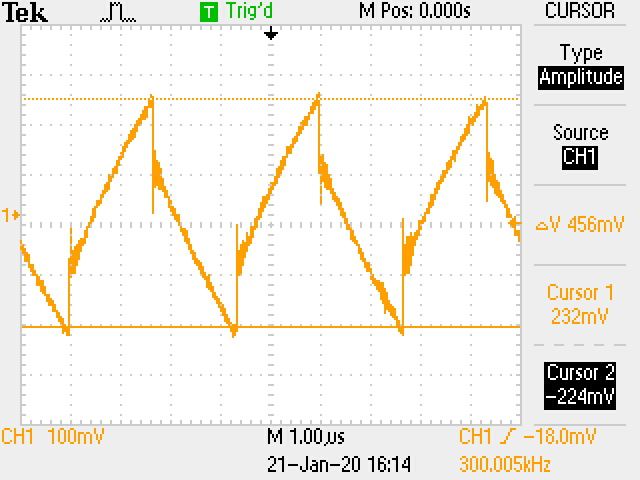
\includegraphics[width=0.6\linewidth]{ALL0002/F0002TEK}
	\caption{Effects of the square wave input.}
	\label{fig:square}
\end{figure}



\pagebreak

\section{Low-pass RL circuit}
\subsection{Purpose}
This experiment demonstrated a resistor-inductor (RL) circuit, which was characterized by a transfer function. 
\subsection{Theoretical background}
The circuit diagram used in this experiment is shown below in Figure \ref{fig:rl}. As this follows a voltage divider, we find the output voltage as, 
\begin{equation}
	\mathbf{V}_o = \frac{1}{1 + j \frac{L}{R} \omega} \mathbf{V}_i
\end{equation}
At low frequencies ($\omega \to 0$), the output voltage is equal to the input. At higher frequencies ($\omega \to \infty$), the impedance due to the inductor is maximized and the input is filtered. This becomes an STC low-pass filter. The 3dB frequency is given as $\omega_0 = L/R$ and the time constant $\tau$ will be the inverse of this. 

For the components $R=\SI{300}{\ohm}$ and $L=\SI{1}{\milli\henry}$ with \SI{50}{\ohm} source resistance, we can simulate this using SPICE. The result the frequency response (AC sweep) simulation is shown in Figure \ref{fig:rlsim} (Appendix). Next, the transient response was found in order to find the time constant for the circuit, shown in Figure \ref{fig:rlsimtrans} (Appendix). Using cursors in ORCAD, the time constant was determined by the time delta to $0.632*\mathrm{MAX}(V)$ and inverting. The time constant from the simulation was found to be $\tau=\SI{2.89}{\micro\second}$.



\subsection{Procedure}

\begin{enumerate}
	\item The circuit, shown in Figure \ref{fig:rl}, was constructed and the actual resistor and inductor values were recorded.
	\item The function generator output was connected to the input $V_i$ of the circuit and a sine wave was enabled at \SI{10}{\Hz}, \SI{4}{\V} (zero to peak). The frequency was increased periodically until it was near the expected 3dB frequency. At every interval, the input, output, and the gain was recorded. 
	\item When the gain was near the 3dB cutoff, several additional points within the vicinity of the cutoff frequency were recorded.
	\item Next, the function generator was switched to a square wave at $f=\SI{25}{\kHz}$ to find the step response of the circuit. This frequency was chosen as it gave ample time for the RL circuit to reach a maximum, per the simulation.
\end{enumerate}

\begin{figure}[h]
	\centering
	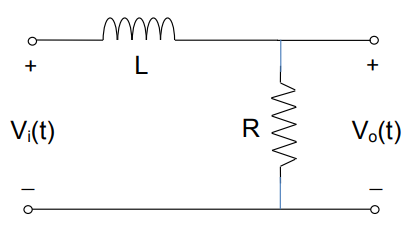
\includegraphics[width=0.4\linewidth]{rl}
	\caption{The low-pass RL circuit used in this experiment.}
	\label{fig:rl}
\end{figure}

\subsection{Results and analysis}
The measured element values were recorded in Table \ref{table:3actual}. There was no known tolerance associated the inductor, but it was within 5\%.

The 3 dB response was found to be roughly \SI{47.3}{\kHz}, roughly \SI{2}{\kHz} from the expected frequency. This $4.23\%$ error is likely due to the real-world values for the unaccounted impedances in the circuit. The data collected is shown in the bode plot in Figure \ref{fig:rlresponse}. Next, the step response using the square wave allowed the time constant to be found as $\tau=\SI{2.840}{\micro\second}$, roughly $1.7\%$ error from the SPICE simulation. The results are summarized in Table \ref{table:3results}.

\subsection{Conclusion}
This experiment demonstrated a first-order RL circuit. The gain can be calculated as a function of the frequency. From this, we can characterize the use of the RL as a filter, which can be used to attenuate high-frequency signals. By finding the 3dB frequency, we can understand when the filter is effective and when it allows signals to pass through.

\begin{table}[h]
	\centering
	\caption{Measured circuit element values used in this experiment.}
	\begin{threeparttable}
		\label{table:3actual}
		\begin{tabular}{cccc}
			\toprule
			Element & Nominal & Measured & Error (Tolerance) \\
			\midrule
			$R$ & \SI{300}{\ohm} & \SI{323.0}{\ohm} & 7.60\% (10\%) \\
			$L$ & \SI{1}{\milli\henry} & \SI{1.044218}{\milli\henry} & 4.422\% (--) \\
			\bottomrule
		\end{tabular}
	\end{threeparttable}
\end{table}

\begin{table}[h]
	\centering
	\caption{Summary of the experimental values.}
	\begin{threeparttable}
		\label{table:3results}
		\begin{tabular}{cccc}
			\toprule
			& Experimental & Theoretical & Error \\
			\midrule
			3 dB response & \SI{47.3}{\kHz} & \SI{49.3}{\kHz} & $4.23\%$ \\
			Time constant & \SI{2.840}{\us} & \SI{2.890}{\us} & $1.7\%$ \\
			\bottomrule
		\end{tabular}
	\end{threeparttable}
\end{table}

\begin{minipage}{0.55\linewidth}
	\begin{figure}[H]
		\centering
		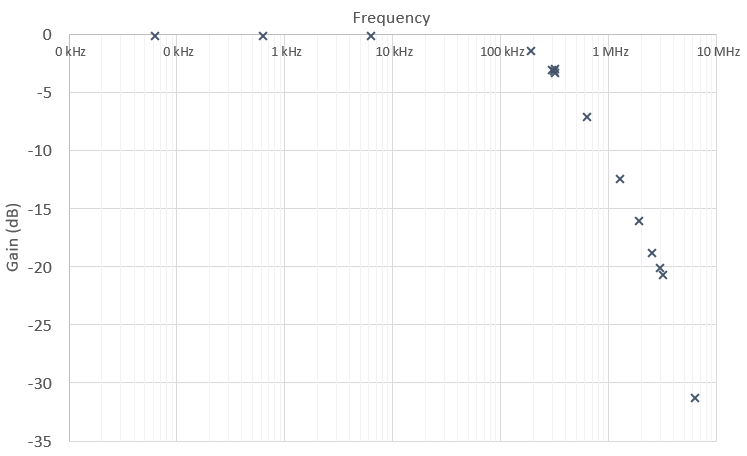
\includegraphics[width=\linewidth]{rlresponse}
		\caption{Response of the RL circuit across $V_o$.}
		\label{fig:rlresponse}
	\end{figure}
\end{minipage}
\begin{minipage}{0.45\linewidth}
\begin{figure}[H]
	\centering
	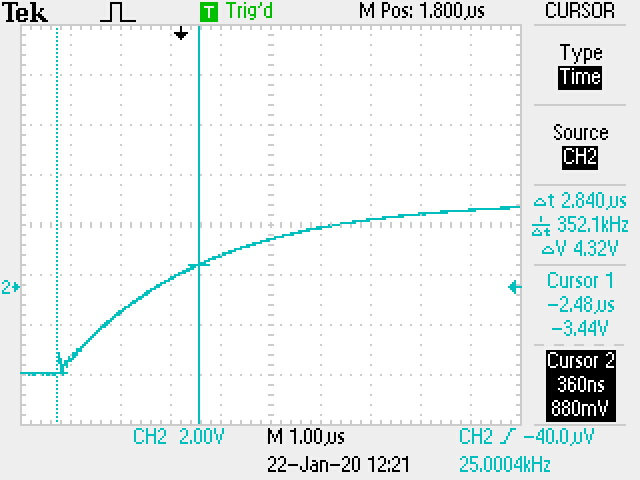
\includegraphics[width=1.0\linewidth]{ALL0011/F0011TEK}
	\caption{Experimental time constant determination using cursors.}
	\label{fig:rltek}
\end{figure}
\end{minipage}
\pagebreak

\section{Oscilloscope characterization}
\subsection{Purpose}
The oscilloscope probes have an impedance that can affect a measurement. In this lab, we will demonstrate the limitations of measuring circuits using the oscilloscope.

\subsection{Theoretical background}
The oscilloscope scopes can be modeled as a parallel resistor capacitor (RC) circuit. The internal resistance is due to an internal shunt. This circuit characteristically has a time constant which can be measured. The oscilloscope probe has a switch that can allow the user to adjust the impedance, listed in Table \ref{table:probes}. The RC circuit that models the probes is shown in Figure \ref{fig:rccircuit}.

We can simulate the effects of the oscilloscope probes in SPICE. First, the cutoff frequency was determined by using a finding the frequency response (AC sweep) of the low-pass circuit. Next, the time constant was found using a transient (step) response on the circuit. Both of these results are shown in Table \ref{table:probes}. Plots of the frequency and step response are shown in Figures \ref{fig:exp4c1x}--\ref{fig:exp4d10x} (Appendix).

\begin{table}[h]
	\centering
	\caption{Impedances of the two probes, as listed in their manuals, and their respective simulated 3dB frequency and time constant.}
	\begin{threeparttable}
		\label{table:probes}
		\begin{tabular}{c|cc|cc}
			\toprule
			Probe & Resistance & Capacitance & 3dB freq. & Time constant $\tau$\\
			\midrule
			X1 & \SI{1}{\mega\ohm} & \SI{95}{\pF} & \SI{14.89}{\kHz} & \SI{8.636}{\us} \\
			X10 & \SI{10}{\mega\ohm} & \SI{16}{\pF} & \SI{93.20}{\kHz} & \SI{1.590}{\us} \\
			\bottomrule
		\end{tabular}
	\end{threeparttable}
\end{table}

\begin{figure}[h]
	\centering
	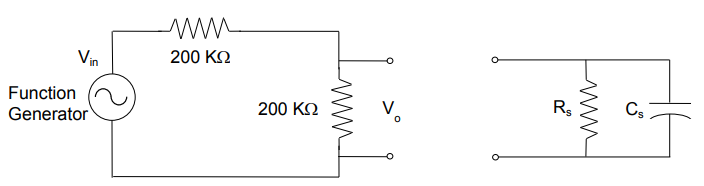
\includegraphics[width=0.7\linewidth]{rccircuit}
	\caption{Left: the voltage divider circuit used to test the oscilloscope probe impedances. Right: an RC circuit modeling the oscilloscope probes.}
	\label{fig:rccircuit}
\end{figure}
\subsection{Procedure}
\begin{enumerate}
	\item The circuit shown in Figure \ref{fig:rccircuit} was constructed and the values of the resistors were collected. The 1X probe was calibrated using the oscilloscope \SI{5}{\V} test output.
	\item The function generator was set to output a sine wave with \SI{8}{\Vpp}. The frequency was swept from \SI{100}{\Hz} to \SI{1}{\MHz}. The outputs were measured using the 1X probe. As the frequency neared a \SI{-3}{\dB} gain, the frequency sweep increments was slowed down to more precisely get a $w_o$ value.
	\item Using a square wave input, the step response was measured of the 1X probe.
	\item Steps 1-4 were repeated using the 10X probe.
\end{enumerate}
\subsection{Results and analysis}
The actual resistor values were recorded in Table \ref{table:4actual}. Both resistors were within tolerance.

The 3 dB frequency was found for both the 1X and 10X probes and are recorded in Table \ref{table:1x10xresults}. For this experiment, primarily using the 10X probe, second-order effects were experienced as the function generator is non-ideal. This led to an upward movement, clearly visible on the frequency-gain curve in Figure \ref{fig:1c}. This would likely not be visible if the function generator were calibrated and had lower internal impedance. Due to this, there was a high error, producing 14.9\% and 5.3\% for the 1X and 10X probes respectively.

The time constant was found using a square pulse and the time constants are recorded in Table \ref{table:1x10xresults}. The percent error for the 1X and 10X probe from simulation is $1.5\%$ and $4.4\%$ respectively. The actual curves are shown in Figure \ref{fig:1d}. The second order effects were not visible in this experiment, likely as the square waves were not affected by the earlier impedances. This led to a much lower error and agrees with our theoretical simulated values.

\subsection{Conclusion}
The oscilloscope probes can be characterized as a first-order RC circuit. We can treat the internal shunts as a parallel RC component. Adding a probe to a circuit can induce significant changes to a circuit and can greatly affect a measurement. It can act attenuate high frequency signals, in this case, attenuating signals over \SI{15}{\kHz} for a 1X probe, and \SI{100}{\kHz} for the 10X probe. 


\begin{table}[H]
	\centering
	\caption{Measured resistor values used in this experiment.}
	\begin{threeparttable}
		\label{table:4actual}
		\begin{tabular}{cccc}
			\toprule
			Element & Nominal & Measured & Error (Tolerance) \\
			\midrule
			$R_1$ & \SI{200}{\kohm} & \SI{196.40}{\kohm} & 2.00\% (5\%) \\
			$R_2$ & \SI{200}{\kohm} & \SI{201.65}{\kohm} & 0.83\% (5\%) \\
			\bottomrule
		\end{tabular}
	\end{threeparttable}
\end{table}
\begin{table}[H]
	\centering
	\caption{Both the simulated and experimental results of the RC-model experiment.}
	\begin{threeparttable}
		\label{table:1x10xresults}
		\begin{tabular}{c|cc|cc|cc}
			\toprule
			\multirow{2}{*}{Probe} & \multicolumn{2}{c|}{Simulated} & \multicolumn{2}{c|}{Experimental} & \multicolumn{2}{c}{\% Error} \\
			& 3 dB freq. & Time const. & 3 dB freq. & Time const. & 3 dB freq. & Time const. \\
			\midrule
			X1  & \SI{14.89}{\kHz} & \SI{8.636}{\us} & \SI{17.5}{\kHz} & \SI{8.50}{\us} & 14.9\% & 1.50\% \\
			X10 & \SI{93.20}{\kHz} & \SI{1.590}{\us} & \SI{98.2}{\kHz} & \SI{1.52}{\us} & 5.3\% & 4.4\% \\
			\bottomrule
		\end{tabular}
	\end{threeparttable}
\end{table}

\pagebreak
\hspace{0pt}
\vfill

\begin{figure}[H]
	\begin{minipage}{0.5\linewidth}
		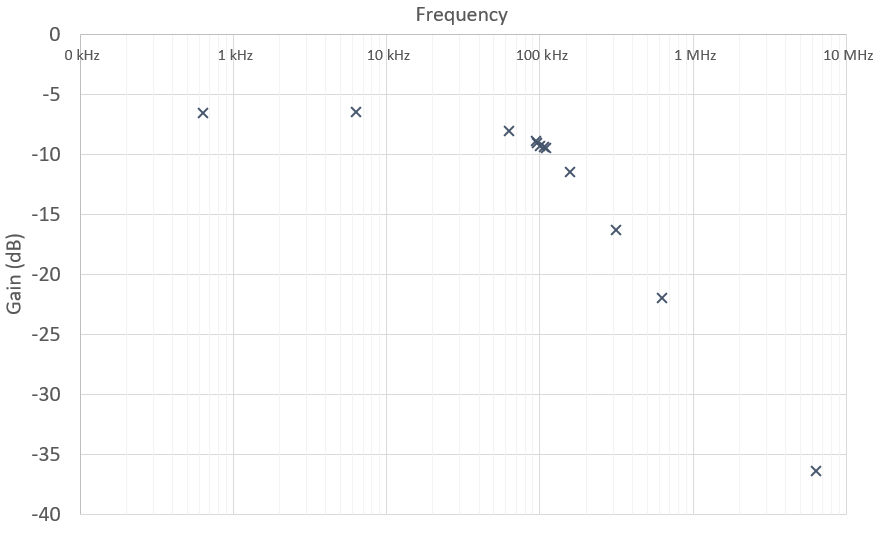
\includegraphics[width=1.0\linewidth]{exp4c1x}
	\end{minipage}
	\begin{minipage}{0.5\linewidth}
		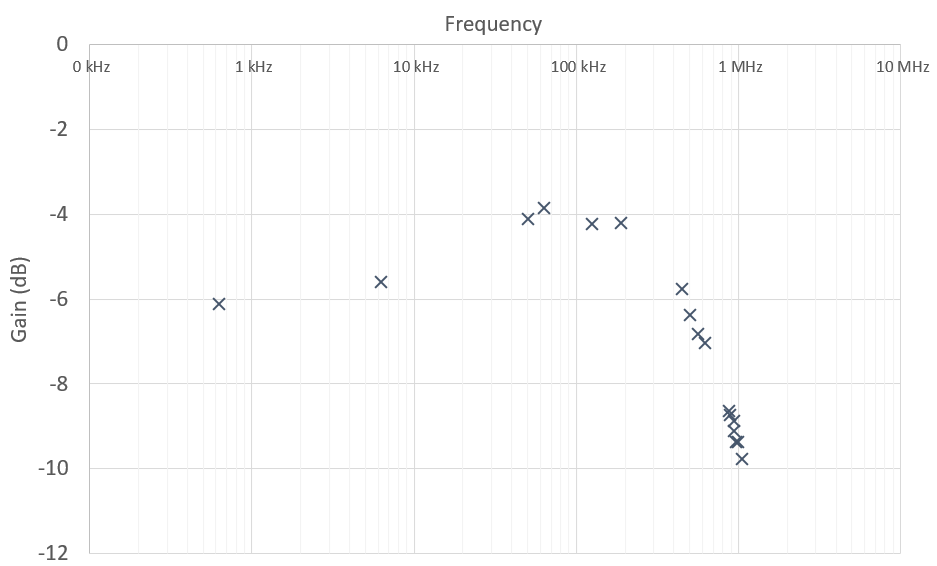
\includegraphics[width=1.0\linewidth]{exp4c10x}
	\end{minipage}
	\caption{The frequency responses of the 1X (left) and 10X probe (right). Note the second-order effects seen in the 10X response, due to a non-ideal function generator.}
	\label{fig:1c}
\end{figure}

\begin{figure}[H]
	\begin{minipage}{0.5\linewidth}
		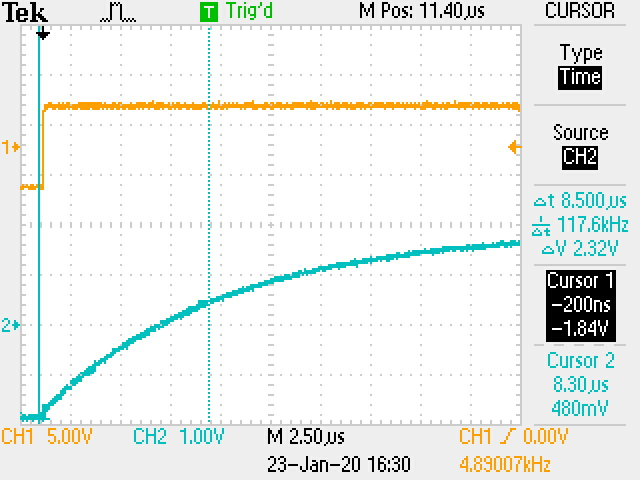
\includegraphics[width=1.0\linewidth]{ALL0012/F0012TEK}
	\end{minipage}
	\begin{minipage}{0.5\linewidth}
		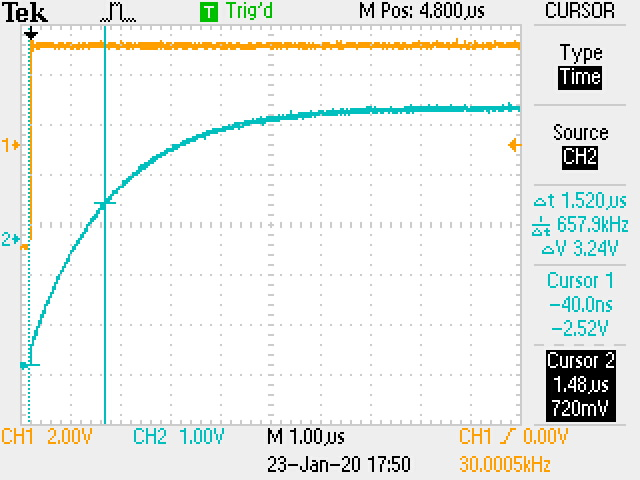
\includegraphics[width=1.0\linewidth]{ALL0014/F0014TEK}
	\end{minipage}
	\caption{The step response of the 1X (left) and 10X (right) oscilloscope probes.}
	\label{fig:1d}
\end{figure}

\vfill
\hspace{0pt}
\pagebreak

\pagebreak

\section*{Appendix}
\vspace{-2em}
\begin{figure}[h]
	\centering
	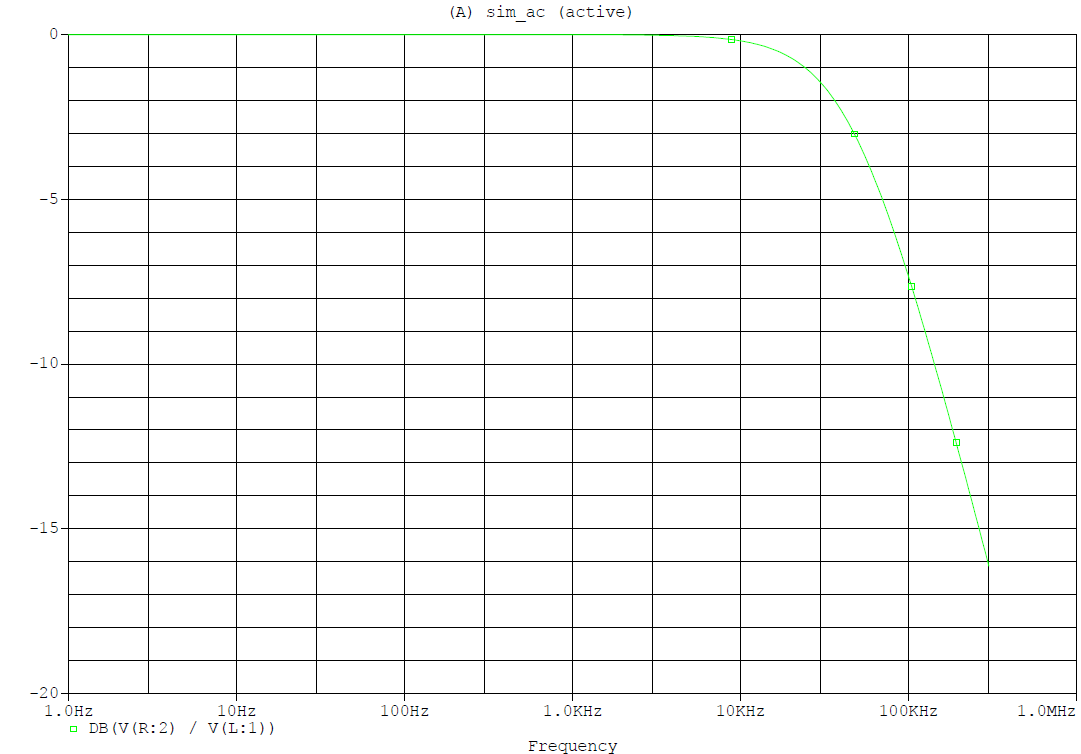
\includegraphics[width=0.65\linewidth]{rlsim}
	\caption{SPICE simulation of the frequency response in Experiment 3.}
	\label{fig:rlsim}
\end{figure}
\begin{figure}[h]
	\centering
	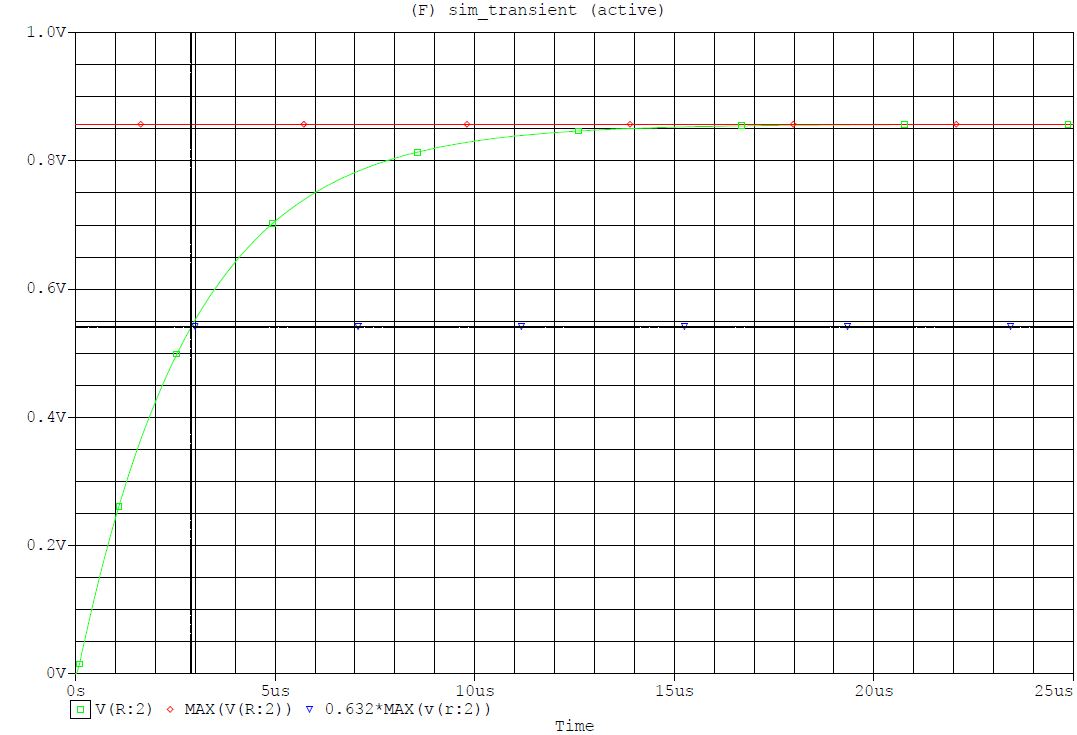
\includegraphics[width=0.65\linewidth]{rlsimtrans}
	\caption{SPICE simulation of the transient response in Experiment 3.}
	\label{fig:rlsimtrans}
\end{figure}
%%%%%
\begin{figure}[h]
	\centering
	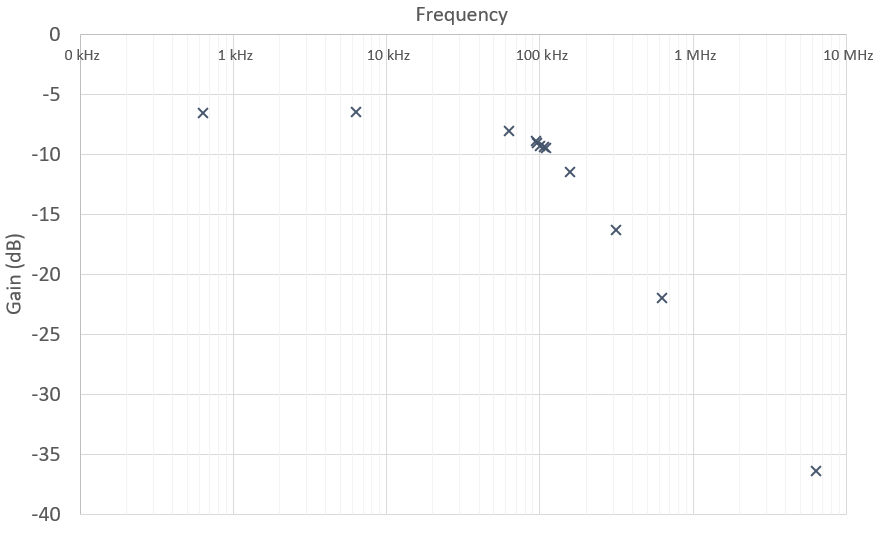
\includegraphics[width=0.7\linewidth]{exp4c1x}
	\caption{Frequency response of the simulated 1X probe.}
	\label{fig:exp4c1x}
\end{figure}

\begin{figure}[h]
	\centering
	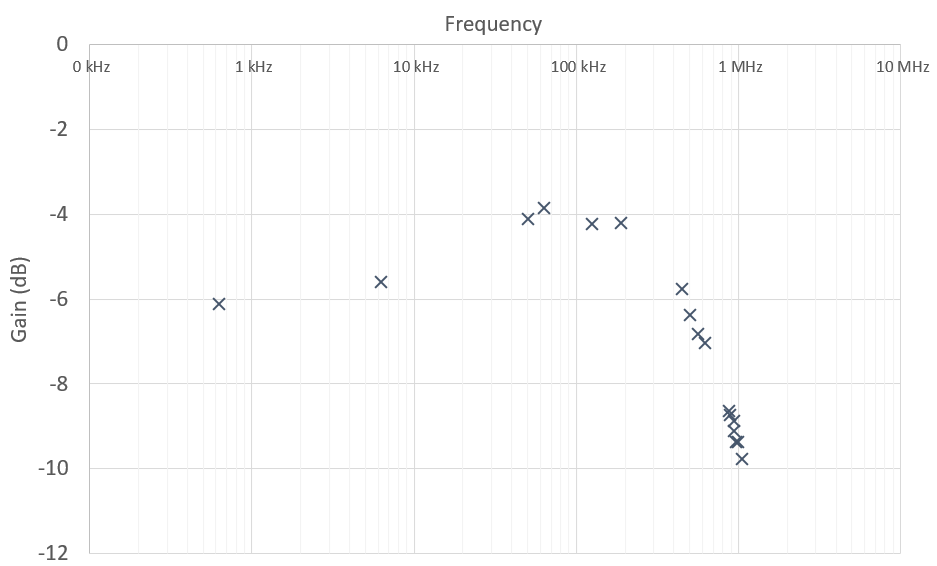
\includegraphics[width=0.7\linewidth]{exp4c10x}
	\caption{Frequency response of the simulated 10X probe.}
	\label{fig:exp4c10x}
\end{figure}

\begin{figure}[h]
	\centering
	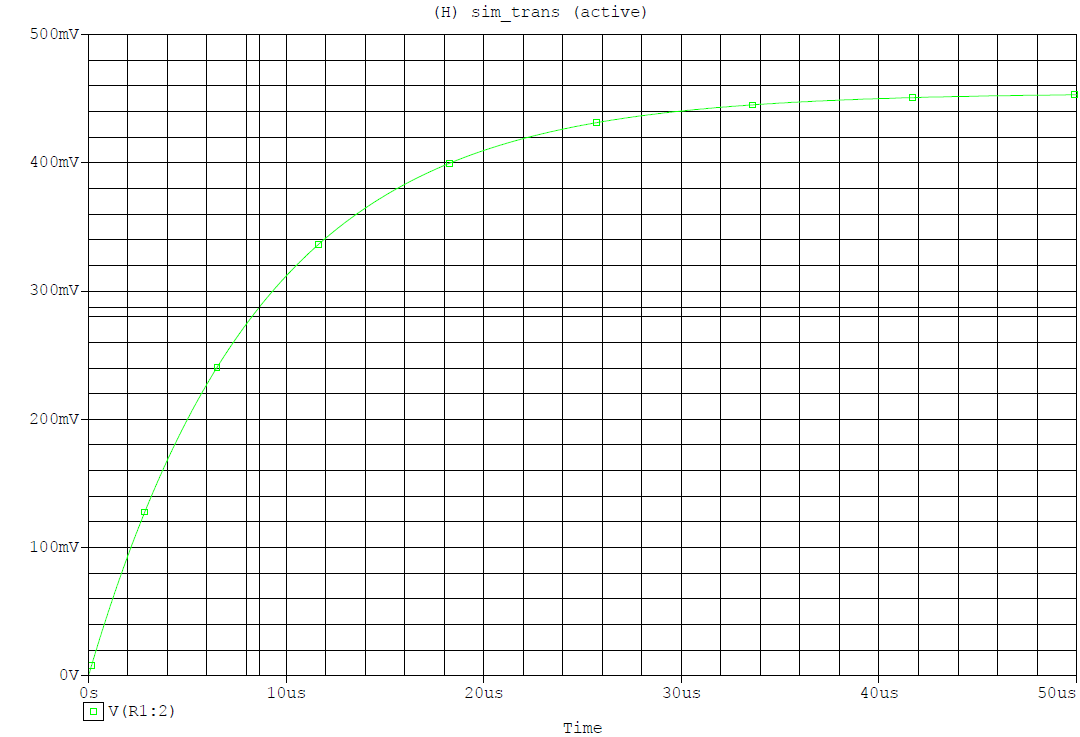
\includegraphics[width=0.7\linewidth]{exp4d1x}
	\caption{Transient/step response of the simulated 1X probe.}
	\label{fig:exp4d1x}
\end{figure}

\begin{figure}[h]
	\centering
	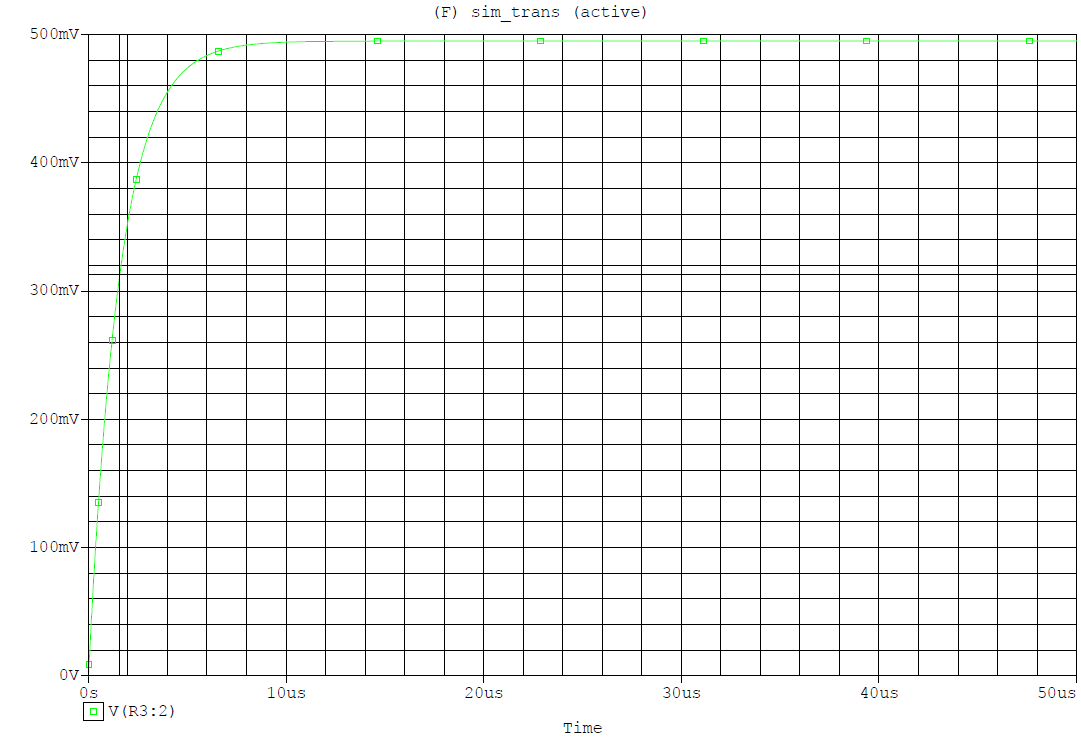
\includegraphics[width=0.7\linewidth]{exp4d10x}
	\caption{Transient/step response of the simulated 10X probe.}
	\label{fig:exp4d10x}
\end{figure}


\end{document}